\documentclass[a4paper, 11pt]{article}

% ======================================================================
% --- PACKAGES ---
% ======================================================================

% --- Language and Fonts ---
\usepackage[utf8]{inputenc}
\usepackage[T1]{fontenc}
\usepackage[english]{babel}
\usepackage{lmodern} % A modern, clean font

% --- Layout and Colors ---
\usepackage[a4paper, margin=2.5cm, headheight=15pt]{geometry}
\usepackage[svgnames]{xcolor} % Defines many colors, e.g., "Crimson"

% --- Packages for Design Elements ---
\usepackage{graphicx}
\usepackage{sectsty} % For styling headings
\usepackage{fontawesome5} % For icons like \faInfoCircle
\usepackage{tikz} % For diagrams
\usetikzlibrary{shapes, arrows, positioning}
\usepackage{dirtree} % For displaying directory trees

% --- Colored Boxes and Code Listings ---
\usepackage[most]{tcolorbox}
\usepackage{listings}

% --- Hyperlinks ---
\usepackage[colorlinks=true, urlcolor=Crimson, linkcolor=Crimson]{hyperref}


% ======================================================================
% --- CUSTOM DEFINITIONS AND STYLES ---
% ======================================================================

% --- Color Palette ---
\definecolor{RPIRed}{HTML}{C51A4A}
\definecolor{RPIBlue}{HTML}{4A74C5}
\definecolor{RPIGray}{HTML}{5D5D5D}
\definecolor{CodeBackground}{HTML}{F5F5F5}

% --- Heading Style ---
\sectionfont{\sffamily\bfseries\color{RPIRed}}
\subsectionfont{\sffamily\bfseries\color{RPIGray}}
\subsubsectionfont{\sffamily\bfseries\color{RPIBlue}}

% --- Configuration for Code Blocks (listings) ---
% KORREKTUR: Fehlende Schlüssel-Wert-Paare hinzugefügt
\lstdefinestyle{cstyle}{
	backgroundcolor=\color{CodeBackground},   
	commentstyle=\itshape\color{Green},
	keywordstyle=\bfseries\color{RPIBlue},
	numberstyle=\tiny\color{RPIGray},
	stringstyle=\color{RPIRed},
	basicstyle=\ttfamily\footnotesize,
	breakatwhitespace=false,         
	breaklines=true,                 
	captionpos=b,                    
	keepspaces=true,                 
	numbers=left,                    
	numbersep=5pt,                  
	showspaces=false,                
	showstringspaces=false,
	showtabs=false,                  
	tabsize=2,
	language=C
}

% --- Configuration for Info Boxes (tcolorbox) ---
\newtcolorbox{infobox}[2][]{
	colback=blue!5!white,
	colframe=RPIBlue!75!black,
	fonttitle=\bfseries,
	title=#2,
	#1,
}

\newtcolorbox{warningbox}[2][]{
	colback=red!5!white,
	colframe=RPIRed!75!black,
	fonttitle=\bfseries,
	title=#2,
	#1,
}

% ======================================================================
% --- TITLE PAGE ---
% ======================================================================
\title{\sffamily\bfseries\Huge OhneBS Operating System\\
	\large \vspace{1em} Documentation Version 0.2.0}
\author{\href{mailto:marwin@zoepfel.de}{Marwin Zöpfel}}
\date{\today}


% ======================================================================
% --- DOCUMENT CONTENT ---
% ======================================================================
\begin{document}
	
	\maketitle
	\thispagestyle{empty}
	\newpage
	
	\tableofcontents
	\newpage
	
	\section{Introduction and Concept}
	This document describes the architecture and functionality of the bare-metal operating system "OhneBS," version 0.2.0.
	
	The term "bare-metal" signifies that this operating system runs directly on the Raspberry Pi hardware, without the assistance of an underlying OS like Linux. Every aspect, from controlling hardware pins to processing user input, must be implemented from scratch.
	
	\begin{infobox}{Project Objective}
		The primary goal of OhneBS is to learn the fundamental concepts of low-level hardware programming and operating system development, and to create a simple yet functional interactive system.
	\end{infobox}
	
	Version 0.2.0 implements a serial command-line interface (shell) that enables variable management and basic arithmetic. Additionally, it introduces basic graphics capabilities on the Raspberry Pi's framebuffer.
	
	\section{Architecture and Project Structure}
	OhneBS adheres to the principle of modularization. The architecture is divided into distinct layers to ensure a clean separation of responsibilities.
	
	\subsection{Architecture Diagram}
	The following diagram illustrates the dependencies between the software layers:
	
	\begin{center}
		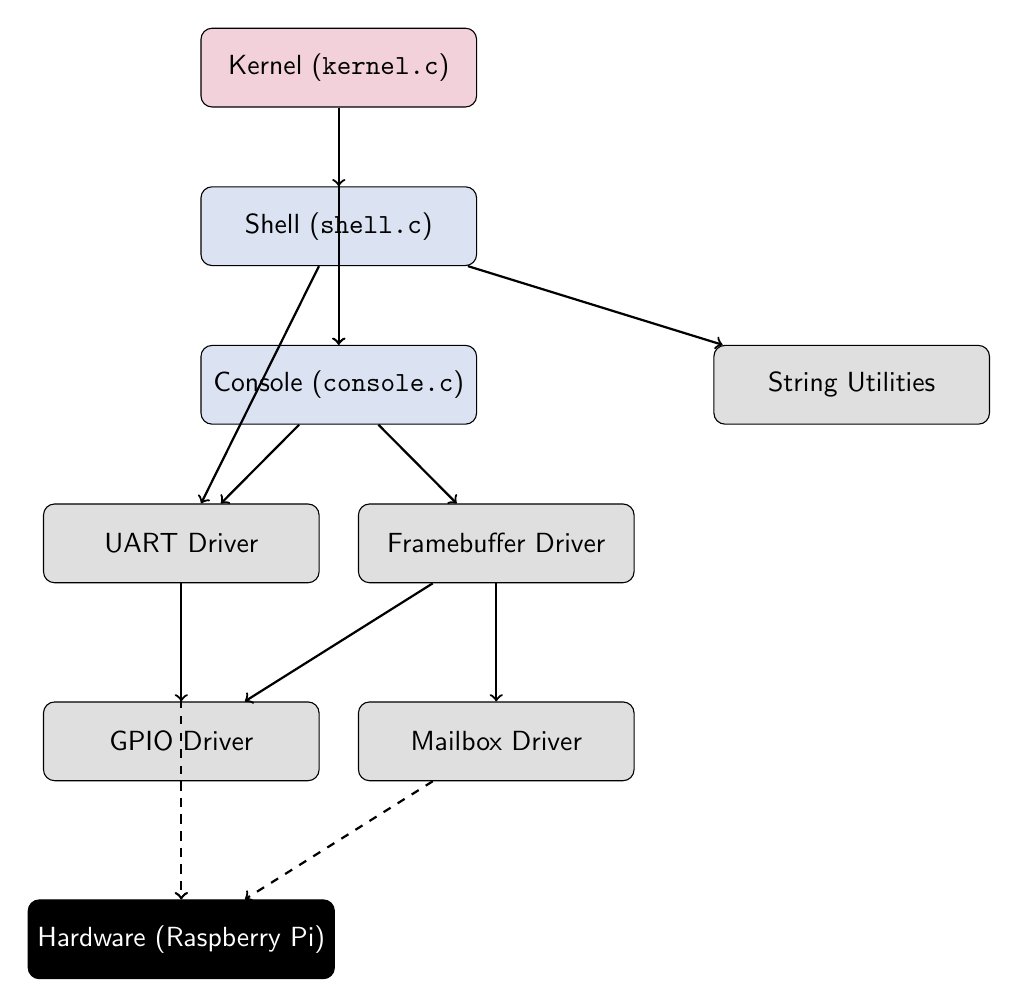
\begin{tikzpicture}[
			node distance=1cm,
			box/.style={rectangle, draw, minimum height=1cm, minimum width=3.5cm, text centered, rounded corners, font=\sffamily},
			]
			\node (kernel) [box, fill=RPIRed!20] {Kernel (\texttt{kernel.c})};
			\node (shell) [box, below=of kernel, fill=RPIBlue!20] {Shell (\texttt{shell.c})};
			\node (console) [box, below=of shell, fill=RPIBlue!20] {Console (\texttt{console.c})}; % New Console module
			\node (uart) [box, below=of console, xshift=-2cm, fill=RPIGray!20] {UART Driver};
			\node (fb) [box, below=of console, xshift=2cm, fill=RPIGray!20] {Framebuffer Driver}; % New Framebuffer module
			\node (gpio) [box, below=of uart, yshift=-0.5cm, fill=RPIGray!20] {GPIO Driver};
			\node (mb) [box, below=of fb, yshift=-0.5cm, fill=RPIGray!20] {Mailbox Driver}; % New Mailbox module
			\node (utils) [box, right=of console, xshift=2cm, fill=RPIGray!20] {String Utilities};
			\node (hw) [box, below=of gpio, yshift=-0.5cm, fill=black, text=white] {Hardware (Raspberry Pi)};
			
			\draw[->, thick] (kernel) -- (shell);
			\draw[->, thick] (kernel) -- (console); % Kernel uses Console
			\draw[->, thick] (shell) -- (console); % Shell uses Console
			\draw[->, thick] (shell) -- (uart); % Shell still reads from UART directly
			\draw[->, thick] (shell) -- (utils);
			\draw[->, thick] (console) -- (uart); % Console uses UART
			\draw[->, thick] (console) -- (fb); % Console uses Framebuffer
			\draw[->, thick] (uart) -- (gpio);
			\draw[->, thick] (fb) -- (gpio); % Framebuffer uses GPIO
			\draw[->, thick] (fb) -- (mb); % Framebuffer uses Mailbox
			\draw[->, thick, dashed] (gpio) -- (hw);
			\draw[->, thick, dashed] (uart) -- (hw);
			\draw[->, thick, dashed] (mb) -- (hw); % Mailbox interacts with hardware
		\end{tikzpicture}
	\end{center}
	
	\newpage
	
	\subsection{Directory Tree}
	The physical structure on the disk reflects the logical separation.
	% KORREKTUR: Unterstriche in Dateinamen müssen escaped werden.
	\dirtree{%
		.1 OhneBS/.
		.2 build/.
		.2 include/.
		.3 console.h.
		.3 fb.h.
		.3 gpio.h.
		.3 mb.h.
		.3 shell.h.
		.3 string\_utils.h.
		.3 uart.h.
		.2 src/.
		.3 boot.S.
		.3 console.c.
		.3 fb.c.
		.3 gpio.c.
		.3 kernel.c.
		.3 mb.c.
		.3 shell.c.
		.3 string\_utils.c.
		.3 uart.c.
		.2 LICENSE.
		.2 link.ld.
		.2 Makefile.gcc.
		.2 Readme.md.
	}
	
	% ======================================================================
	% --- NEUER ABSCHNITT: BOOT PROCESS AND KERNEL INITIALIZATION (KORRIGIERT) ---
	% ======================================================================
	
	\newpage
	\section{Boot Process and Kernel Initialization}
	This section provides a detailed, step-by-step walkthrough of the entire process that brings OhneBS to life, from the moment the Raspberry Pi is powered on to the execution of the main kernel loop.
	
	\subsection{The Black Box: The Firmware Stage}
	The very first moments of the boot process are controlled by proprietary firmware stored in the Raspberry Pi's on-chip ROM. This stage is a "black box" for our operating system, but it's crucial to understand what it does for us.
	\begin{enumerate}
		\item \textbf{Power On:} The ARM cores are initially off. The VideoCore IV GPU is the first component to start.
		\item \textbf{First Stage Bootloader:} The GPU executes code from its internal ROM, which mounts the SD card and looks for the file \texttt{bootcode.bin}.
		\item \textbf{Second Stage Bootloader:} \texttt{bootcode.bin} is loaded into the GPU's L2 cache and executed. Its primary job is to initialize the SDRAM, allowing the larger third-stage bootloader to be loaded.
		\item \textbf{Third Stage Bootloader (\texttt{start.elf}):} This is the main GPU firmware. It reads the \texttt{config.txt} file to configure various hardware parameters (like clock speeds, HDMI settings, etc.). Its final and most important task for us is to look for our kernel image file, \texttt{kernel8.img}, load it into SDRAM at the physical address \texttt{0x80000}, and finally, "wake up" the primary ARM CPU core (Core 0) and instruct it to start executing code at that address.
	\end{enumerate}
	
	\begin{infobox}{\faKey\ The Handoff}
		The moment \texttt{start.elf} finishes and points the ARM core's Program Counter to \texttt{0x80000} is the magical handoff. From this point on, the proprietary firmware is out of the picture, and \textbf{the OhneBS code has full control} of the machine.
	\end{infobox}
	
	\subsection{The Kernel Stage: From Assembly to C}
	Execution now begins at the very first instruction in our own code, defined by the \texttt{\_start} label in the \texttt{boot.S} assembly file.
	
	\subsubsection{Step 1: Core Verification}
	The Raspberry Pi 400 has a quad-core CPU. The firmware only starts Core 0. It's our responsibility to handle the other cores. The first thing we do is check which core is executing our code.
	
	% KORREKTUR: language=Assembler zu   geändert
	\begin{lstlisting}[style=cstyle, language={}, caption={Checking the core ID in \texttt{boot.S}}]
		// Read the Multiprocessor Affinity Register (MPIDR_EL1)
		mrs     x1, mpidr_el1
		// Isolate the last two bits, which contain the core ID (0-3)
		and     x1, x1, #3
		// If the result is zero (it's Core 0), branch to the main setup
		cbz     x1, 2f
		
		// We're not on the main core, so hang in an infinite wait loop
		1:  wfe
		b       1b
		2:  // We're on the main core! Continue...
	\end{lstlisting}
	This ensures that only the primary core proceeds to initialize the kernel. The other cores are put into a low-power sleep state using the `wfe` (Wait For Event) instruction.
	
	\subsubsection{Step 2: Stack Initialization}
	Before we can call any functions (especially C functions), we need a stack. The stack is a region of memory used for local variables, function parameters, and return addresses. We initialize the Stack Pointer register (`sp`) to point to the beginning of our kernel code. Since the stack on ARM grows downwards, this gives us the memory space *below* our code to use as a temporary stack.
	
	% KORREKTUR: language=Assembler zu   geändert
	\begin{lstlisting}[style=cstyle, language={ }, caption={Setting up the initial stack pointer.}]
		// Set stack to start at the beginning of our code
		ldr     x1, =_start
		mov     sp, x1
	\end{lstlisting}
	
	\subsubsection{Step 3: Clearing the BSS Section}
	% KORREKTUR: Unterstriche mit \ escaped
	In C, global or static variables that are not explicitly initialized are guaranteed to be zero. The compiler doesn't store these zeros in the image file. Instead, it groups all such variables into a memory region called the "BSS section" and provides two symbols: \texttt{\_\_bss\_start} and \texttt{\_\_bss\_size}. It is the operating system's job to manually write zeros to this entire memory region before any C code runs.
	
	% KORREKTUR: language=Assembler zu   geändert
	\begin{lstlisting}[style=cstyle, language={ }, caption={Zeroing out the BSS section.}]
		// Clean the BSS section
		ldr     x1, =__bss_start     // Start address
		ldr     w2, =__bss_size      // Size of the section
		3:  cbz     w2, 4f               // Quit loop if size is zero
		str     xzr, [x1], #8        // Store a 64-bit zero and increment address
		sub     w2, w2, #1           // Decrement size counter (in 8-byte chunks)
		cbnz    w2, 3b               // Loop if non-zero
	\end{lstlisting}
	
	% KORREKTUR: Unterstrich mit \ escaped
	\subsubsection{Step 4: The Jump to C (\texttt{kernel\_main})}
	% KORREKTUR: Unterstrich mit \ escaped
	With the low-level setup complete, the assembly code performs its final task: it calls our main C function, \texttt{kernel\_main}. The `bl` (Branch with Link) instruction jumps to the C code and also stores the return address in a register, although our \texttt{kernel\_main} function is designed to never return.
	
	% KORREKTUR: language=Assembler zu   und livedlisting zu lstlisting geändert
	\begin{lstlisting}[style=cstyle, language={ }, caption={Calling the C kernel.}]
		// Jump to our main() routine in C
		4:  bl      kernel_main
	\end{lstlisting}
	
	% KORREKTUR: Unterstrich mit \ escaped
	\subsubsection{Step 5: High-Level Initialization (\texttt{kernel.c})}
	% KORREKTUR: Unterstrich mit \ escaped
	Control is now within the familiar world of C. The \texttt{kernel\_main} function acts as the main orchestrator, initializing all the high-level drivers and services in a specific order.
	
	\begin{lstlisting}[style=cstyle, caption={The entry point of the C kernel.}]
		void kernel_main() {
			// 1. Initialize serial communication for debugging
			uart_init();
			
			// 2. Initialize the shell's internal state
			shell_init();
			
			// 3. Initialize the framebuffer via mailbox calls to the GPU
			fb_init();
			
			// 4. Print a welcome message to the console (now both screen and UART)
			console_puts("Welcome to OhneBS! v0.2.0\n");
			
			// ... (Drawing demo graphics) ...
			
			// 5. Enter the main kernel loop
			while (1) {
				// Continuously poll the shell for updates (e.g., new user input)
				shell_update();
			}
		}
	\end{lstlisting}
	From this point on, the system is fully initialized and has entered its main operational loop, waiting for user input and processing commands. The boot process is complete.
	
	% ======================================================================
	% --- NEUER ABSCHNITT: SHELL AND GPIO DRIVER ---
	% ======================================================================
	
	\section{The Interactive Shell and GPIO Driver}
	
	This section details the highest and lowest levels of the current software stack: the user-facing interactive shell that defines the system's functionality, and the fundamental GPIO driver that communicates with the physical hardware pins.
	
	\subsection{The Interactive Shell (\texttt{shell.c})}
	The shell is the primary user interface of OhneBS. It provides a command-line interface (CLI) that allows a user to interact with and control the kernel.
	
	\subsubsection{Core Logic: The Polling Loop}
	The entire shell is driven by a single function, \texttt{shell\_update()}, which is called continuously from the main kernel loop. This represents a \textbf{polling-based architecture}, where the system actively checks for input instead of waiting for an interrupt.
	
	\begin{lstlisting}[style=cstyle, caption={The main kernel loop, driving the shell.}]
		// in kernel.c
		void kernel_main() {
			// ... initializations ...
			
			console_puts("Welcome to OhneBS!\n> ");
			
			while (1) {
				// The CPU spends all its time repeatedly calling this function.
				shell_update();
			}
		}
	\end{lstlisting}
	
	Inside \texttt{shell\_update()}, the \texttt{uart\_read\_byte()} function is called to check for new characters. If a character is available, it is processed; otherwise, the function returns immediately.
	
	\subsubsection{Input Processing and Command Execution}
	\begin{enumerate}
		\item \textbf{Buffering:} Received characters are stored in a 256-byte static buffer, \texttt{input\_buffer}. The current position is tracked by \texttt{input\_buffer\_pos}.
		\item \textbf{Echoing:} Every printable character is immediately sent back to the `console` module for display, providing instant user feedback.
		\item \textbf{Editing:} The shell supports backspace (`0x08` or `0x7F`) to delete the last character from the buffer and the screen.
		\item \textbf{Execution:} When a carriage return (`r`) is detected, a null terminator (`0`) is appended to the buffer to create a valid C-string. This string is then passed to the \texttt{process\_command()} function. After execution, the input buffer is cleared for the next command.
	\end{enumerate}
	
	\subsubsection{Command Parser (\texttt{process\_command})}
	The parser is a simple implementation that separates the first word of the input string to identify the command. The rest of the string is then passed as arguments.
	
	\begin{infobox}{\faTerminal\ Implemented Commands}
		\begin{itemize}
			\item \textbf{\texttt{help}}: Displays a list of available commands.
			\item \textbf{\texttt{version}}: Prints the current version string of the OS.
			\item \textbf{\texttt{set <name> <value>}}: Creates or updates a named variable with a given integer value. The shell can store up to 50 variables.
			\item \textbf{\texttt{print <expression>}}: Evaluates a simple expression and prints the result. The current evaluator can handle two terms (numbers or variables) joined by a single `+` operator.
		\end{itemize}
	\end{infobox}
	
	\subsection{The GPIO Driver (\texttt{gpio.c})}
	The GPIO (General Purpose Input/Output) driver is the most fundamental layer for interacting with the physical world outside the SoC. It provides direct control over the Raspberry Pi's header pins.
	
	\subsubsection{Design Philosophy: Generic Register Access}
	Instead of writing separate logic for each type of GPIO operation (set function, set pin, clear pin, set pull-up/down), the driver uses a single, powerful helper function: \texttt{gpio\_call()}.
	
	\begin{warningbox}{\faCog\ Understanding GPIO Registers}
		The BCM2711's GPIO functionality is controlled by writing to specific 32-bit registers. For example, the \texttt{GPFSELn} registers control the function of a pin (Input, Output, Alt0-5), with 3 bits dedicated to each pin. The \texttt{GPSETn} and \texttt{GPCLRn} registers set or clear pins by writing a `1` to the corresponding bit. The `gpio\_call` function abstracts the complex math needed to find the correct register and bit position for any given pin.
	\end{warningbox}
	
	\begin{lstlisting}[style=cstyle, caption={The generic gpio\_call function.}]
		unsigned int gpio_call(unsigned int pin_number, unsigned int value, 
		unsigned int base, unsigned int field_size, 
		unsigned int field_max) 
		{
			unsigned int field_mask = (1 << field_size) - 1;
			
			// Calculate which register and which bits within that register to modify
			unsigned int num_fields = 32 / field_size;
			unsigned int reg = base + ((pin_number / num_fields) * 4);
			unsigned int shift = (pin_number % num_fields) * field_size;
			
			// Read-modify-write operation
			unsigned int curval = mmio_read(reg);
			curval &= ~(field_mask << shift); // Clear the relevant bits
			curval |= value << shift;         // Set the new value
			mmio_write(reg, curval);
			
			return 1;
		}
	\end{lstlisting}
	
	\subsubsection{Public API Functions}
	The user-facing functions in \texttt{gpio.h} are simple wrappers around \texttt{gpio\_call()}, providing a clean and readable API.
	
	\paragraph{\texttt{gpio\_function(pin, func)}} Calls \texttt{gpio\_call} with the base address of the \texttt{GPFSEL0} registers and a field size of 3 bits.
	
	\paragraph{\texttt{gpio\_set(pin, val)}} Calls \texttt{gpio\_call} with the base address of the \texttt{GPSET0} registers and a field size of 1 bit.
	
	\paragraph{\texttt{gpio\_pull(pin, val)}} Calls \texttt{gpio\_call} with the base address of the \texttt{GPPUPPDN0} registers and a field size of 2 bits to set pull-up/down states.
	
	
	
	\section{System Execution Flow and I/O Architecture}
	\label{sec:flow}
	
	\subsection{Core Philosophy: From Serial to Screen}
	The initial version of OhneBS relied exclusively on a serial UART connection for all input and output. While robust for debugging, this "headless" approach lacks the immediacy of a real computer system. The primary goal for version 0.2.0 was to enable graphical output on a standard HDMI monitor, providing a persistent, self-contained user interface.
	
	The main challenge is that modern graphics hardware is incredibly complex. Writing a full driver for the HDMI interface from scratch is a monumental task. The Raspberry Pi, however, offers a clever shortcut: a powerful VideoCore IV GPU that handles the low-level hardware communication. The CPU can communicate with the GPU to request services, such as setting up a simple, linear framebuffer.
	
	\begin{infobox}{\faCogs\ The Mailbox Interface}
		A \textbf{framebuffer} is a region of RAM that directly corresponds to the pixels on the screen. Writing a color value to a specific memory address in the framebuffer instantly changes the color of the corresponding pixel. To get the address and configuration of this memory region, our ARM CPU must communicate with the GPU. This is achieved via a \textbf{Mailbox}, a simple message-passing system.
	\end{infobox}
	
	\subsection{The New I/O Data Flow}
	To support both the new framebuffer and the existing UART console, a new abstraction layer, the \textbf{Console Module}, was introduced. This module acts as a central hub for all text output. Higher-level components like the Shell no longer need to know *where* their output is going; they simply send it to the console.
	
	The diagram below illustrates this improved data flow:
	
	\begin{center}
		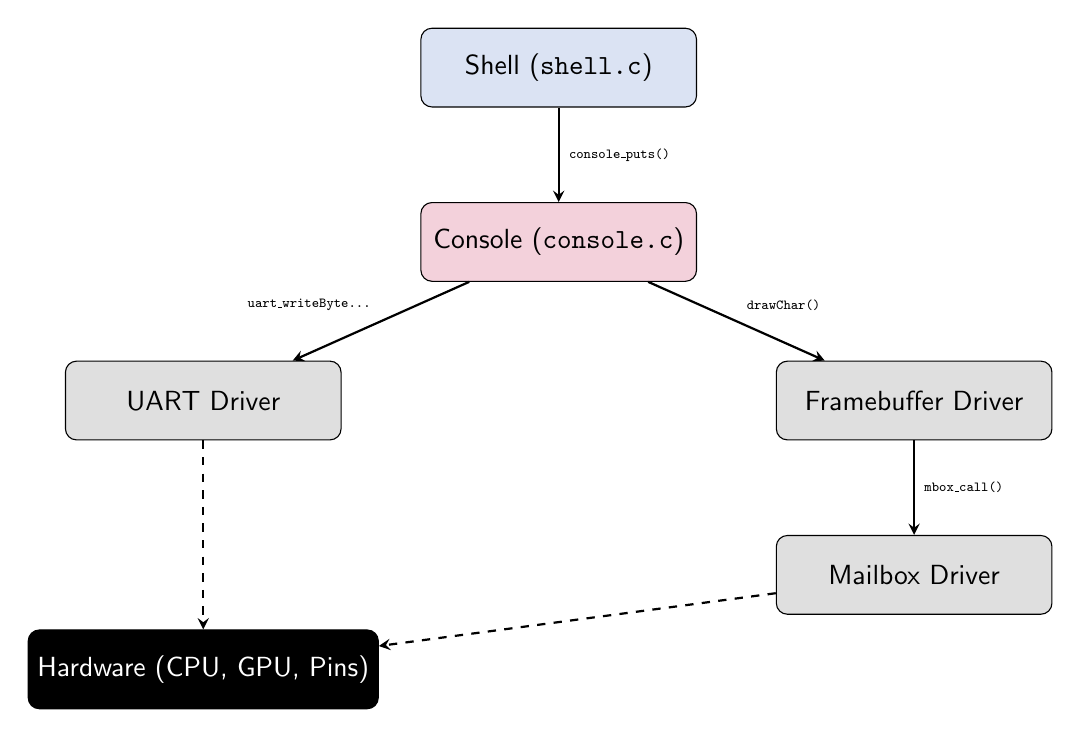
\begin{tikzpicture}[
			node distance=1.2cm,
			box/.style={rectangle, draw, minimum height=1cm, minimum width=3.5cm, text centered, rounded corners, font=\sffamily},
			arrow/.style={->, thick, >=stealth}
			]
			% Nodes
			\node (shell) [box, fill=RPIBlue!20] {Shell (\texttt{shell.c})};
			\node (console) [box, below=of shell, fill=RPIRed!20] {Console (\texttt{console.c})};
			\node (uart) [box, below left=1cm and 1cm of console, fill=RPIGray!20] {UART Driver};
			\node (fb) [box, below right=1cm and 1cm of console, fill=RPIGray!20] {Framebuffer Driver};
			\node (mb) [box, below=of fb, fill=RPIGray!20] {Mailbox Driver};
			\node (hw) [box, below=of uart, yshift=-1.2cm, fill=black, text=white] {Hardware (CPU, GPU, Pins)};
			
			% Arrows
			\draw[arrow] (shell) -- node[right, midway, font=\tiny\sffamily] {\texttt{console\_puts()}} (console);
			\draw[arrow] (console) -- node[above left, midway, font=\tiny\sffamily] {\texttt{uart\_writeByte...}} (uart);
			\draw[arrow] (console) -- node[above right, midway, font=\tiny\sffamily] {\texttt{drawChar()}} (fb);
			\draw[arrow] (fb) -- node[right, midway, font=\tiny\sffamily] {\texttt{mbox\_call()}} (mb);
			
			% Hardware connections
			\draw[arrow, dashed] (uart) -- (hw);
			\draw[arrow, dashed] (mb) -- (hw);
			
			
		\end{tikzpicture}
		\begin{itemize}
			\textbf{Execution Path:}\\
			\textbf{1.} The \texttt{shell} requests to print a string.\\
			\textbf{2.} The \texttt{console} receives the request.\\
			\textbf{3.} It forwards each character to \textbf{both} the \texttt{UART} driver and the \texttt{Framebuffer} driver.\\
			\textbf{4.} The \texttt{Framebuffer} driver itself uses the \texttt{Mailbox} driver during its initialization.
		\end{itemize}
	\end{center}
	
	\newpage
	\section{Module Reference: Implementation Details}
	
	This chapter provides a deeper insight into the implementation of the new and updated modules.
	
	\subsection{Mailbox Module (\texttt{mb.c})}
	This module implements the low-level protocol for communicating with the VideoCore GPU.
	
	\subsubsection{Mechanism}
	The communication relies on a shared memory buffer and a set of hardware registers.
	\begin{enumerate}
		\item A message buffer is prepared in RAM. This buffer must be 16-byte aligned because the GPU only receives the upper 28 bits of the address.
		\item The memory address of this buffer, combined with a channel number, is written to the \texttt{MBOX\_WRITE} register.
		\item The CPU then polls the \texttt{MBOX\_STATUS} register, waiting for the GPU to signal that it has placed a response in the mailbox.
		\item The CPU reads the \texttt{MBOX\_READ} register to confirm the response is for its original message and then processes the data in the shared memory buffer.
	\end{enumerate}
	
	\begin{lstlisting}[style=cstyle, caption={The core of the synchronous mailbox call.}]
		unsigned int mbox_call(unsigned char ch)
		{
			// Combine the 28-bit address of our buffer with the 4-bit channel
			unsigned int r = ((unsigned int)((long) &mbox) &~ 0xF) | (ch & 0xF);
			
			// Wait until the mailbox is not full
			while (mmio_read(MBOX_STATUS) & MBOX_FULL);
			
			// Write our message address to the mailbox
			mmio_write(MBOX_WRITE, r);
			
			while (1) {
				// Wait until the mailbox is not empty (has a reply)
				while (mmio_read(MBOX_STATUS) & MBOX_EMPTY);
				
				// Check if the reply is for our message
				if (r == mmio_read(MBOX_READ)) {
					// Return success if the GPU response code is positive
					return mbox[1] == MBOX_RESPONSE;
				}
			}
			return 0; // Should not be reached
		}
	\end{lstlisting}
	
	\subsection{Framebuffer Module (\texttt{fb.c})}
	This driver uses the Mailbox interface to initialize a linear framebuffer and provides primitive functions for drawing.
	
	% KORREKTUR: Unterstrich escaped
	\subsubsection{Initialization (\texttt{fb\_init})}
	The \texttt{fb\_init} function is a prime example of the mailbox interface in action. It constructs a long message in the global `mbox` array, filling it with various "tags" to request services from the GPU.
	
	\begin{infobox}{Key Mailbox Tags Used}
		% KORREKTUR: Unterstriche escaped
		\begin{itemize}
			\item \texttt{MBOX\_TAG\_SETPHYWH}: Requests a specific physical screen resolution (e.g., 1920x1080).
			\item \texttt{MBOX\_TAG\_SETDEPTH}: Requests a specific color depth (32 bits per pixel).
			\item \texttt{MBOX\_TAG\_GETFB}: The most important tag. It asks the GPU to allocate the framebuffer memory and return its address and size.
			\item \texttt{MBOX\_TAG\_GETPITCH}: Asks for the "pitch," which is the number of bytes per row on the screen. This is crucial for calculating pixel offsets correctly.
		\end{itemize}
	\end{infobox}
	
	% KORREKTUR: Unterstrich escaped
	After a successful \texttt{mbox\_call}, the GPU-provided physical address is converted to an ARM-accessible address, and the screen parameters (width, height, pitch) are stored for later use.
	
	\subsubsection{Drawing Pixels (\texttt{drawPixel})}
	This is the most fundamental drawing function. All other graphics primitives (`drawLine`, `drawRect`, etc.) are built upon it. It calculates the memory offset for a given (x, y) coordinate and writes a 32-bit color value to that location.
	
	\begin{lstlisting}[style=cstyle, caption={Calculating the memory offset for a pixel.}]
		void drawPixel(int x, int y, unsigned char attr)
		{
			// The pitch is the number of bytes to get to the next row.
			// Each pixel is 4 bytes wide (32-bit color).
			int offs = (y * pitch) + (x * 4);
			
			// Write the 32-bit color value directly to the framebuffer memory.
			// 'vgapal' is an array that maps the 4-bit color attribute to a 32-bit color.
			*((unsigned int*)(fb + offs)) = vgapal[attr & 0x0f];
		}
	\end{lstlisting}
	
	\subsection{Console Abstraction Module (\texttt{console.c})}
	This new module provides a unified text output interface, decoupling the shell from the physical display hardware.
	
	\subsubsection{Dual Output}
	% KORREKTUR: Unterstriche escaped und \item in enumerate-Umgebung
	The core of this module is the \texttt{console\_putc} function. It acts as a multiplexer, sending every single character to two destinations:
	\begin{enumerate}
		\item \textbf{To the UART Driver:} via \texttt{uart\_writeByteBlocking(c)}. This ensures that all output is still visible on the serial debug console.
		\item \textbf{To the Framebuffer Driver:} via \texttt{drawChar(...)}. This renders the character graphically on the screen.
	\end{enumerate}
	This dual-output approach is invaluable for debugging; even if the graphical output fails, the serial log remains functional.
	
	\subsubsection{Cursor Management and Scrolling}
	% KORREKTUR: Unterstriche escaped und \item in itemize-Umgebung
	The console maintains static variables \texttt{current\_x} and \texttt{current\_y} to track the cursor position on the screen. It handles special characters:
	\begin{itemize}
		\item \texttt{\textbackslash n} (Newline): Triggers the \texttt{console\_newline()} helper function.
		\item \texttt{\textbackslash r} (Carriage Return): Resets \texttt{current\_x} to 0.
		\item \texttt{\textbackslash b} (Backspace): Moves the cursor back and overwrites the character with a background-colored rectangle.
	\end{itemize}
	
	\begin{warningbox}{\faExclamationTriangle\ Current Scrolling Implementation}
		The scrolling mechanism in version 0.2.0 is very basic. When the cursor reaches the bottom of the screen, the entire framebuffer is cleared, and the cursor is reset to the top-left corner (0,0). A future version should implement a more efficient `memcpy`-style operation to scroll the existing content up, providing a smoother user experience.
	\end{warningbox}
	
\end{document}
